% Na zvoleném českém korpusu vyhodnoťte přesnost a pokrytí pravidel. Diskutujte míru, se kterou je možné generovat gramatické věty, a kvalitu textu (přirozené vyjadřování, nezamýšlené vedlejší efekty).

\section{Evaluation Corpus}

For evaluation, I have constructed my own text corpus. The corpus is composed of texts written by contemporary Czech authors who provided the texts themselves. The corpus is intentionally small as humans did the evaluation, and evaluating a large set of sentences would be expensive.

In selecting the texts, I tried to capture various characteristics of the texts. Thus, the corpus consists of several different literary genres; the narrators are both male and female; I have included texts written in the present and past tense, and I have chosen texts containing different types of speech. (Such as direct speech, semi-direct speech...) Finally, the corpus, of course, includes both first-person and third-person narratives.

In total, the evaluation data consists of 36 different texts composed of 388 sentences. The numbers divided by narratives are captured in chart \ref{fig:eval-input-numbers}.

\begin{figure}[!ht]
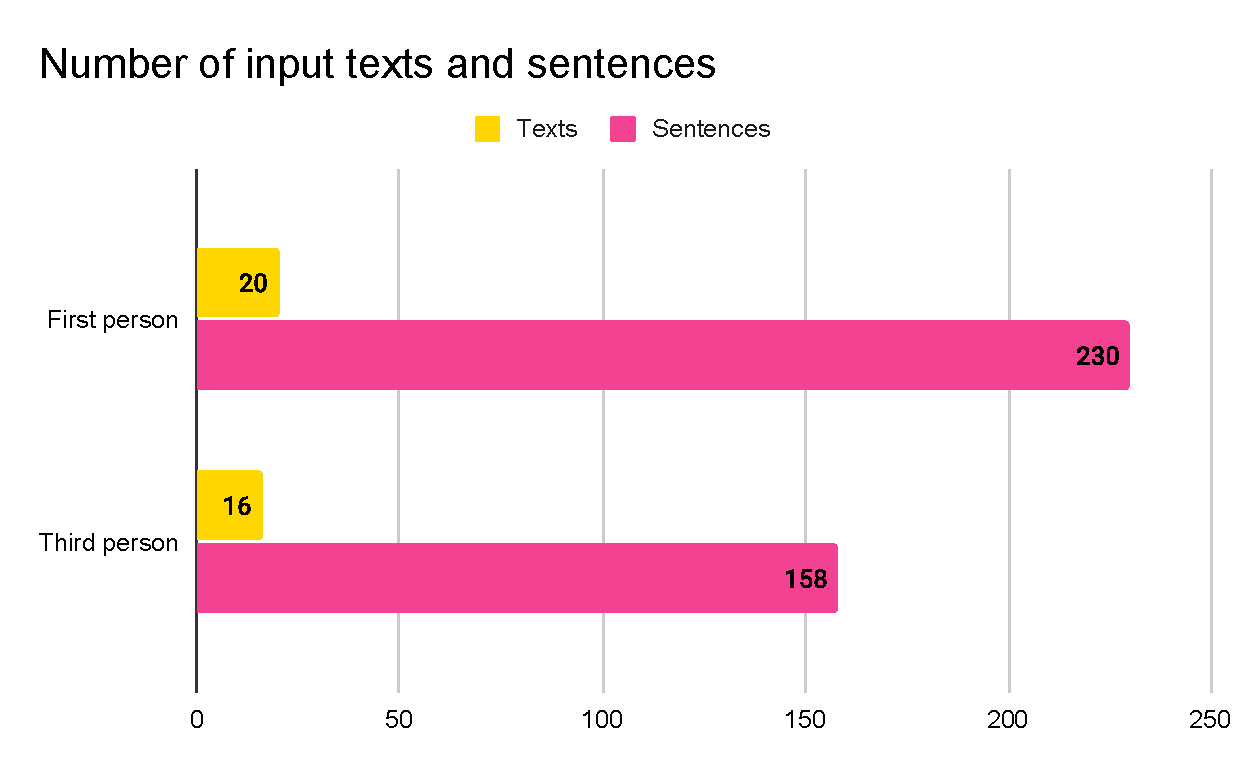
\includegraphics[width=\textwidth]{data/Eval-Input-Numbers.pdf}
\caption{Statistics about the corpus}
\label{fig:eval-input-numbers}
\end{figure}

\section{Annotation Process}

As mentioned in the previous section, human annotators evaluated the sentences manually. The annotators have got: the person the text is converted from, the name of the protagonist, the original text, and the rephrased text. After reading the texts, an annotator could mark one or more statements for each sentence as true.

The possible statements to mark:

\begin{itemize}
	\item The sentence is converted correctly, without grammatical errors, sounds natural, and is unambiguous.
	\item The sentence has lost its unambiguity.
	\item The word order is unnatural, or there are other unnatural sounding elements in the sentence.
	\item The sentence contains grammatical errors.
	\item Some parts of the sentence are converted correctly, and some are not.
	\item The sentence is not converted correctly or not converted at all.
	\item The sentence has not been converted, and that is correct.
\end{itemize}

The evaluation's non-binarity also offers a basic error analysis, which gives us a basis for discussion about the quality of generated texts.

\section{Results}

Based on the marking, I retrieved the results statistics.

As can be seen in figure \ref{fig:eval-total}, most of the sentences were converted correctly, which also includes not converting the sentence at all (about 66\%). Only 17\% of the 388 sentences were converted incorrectly, partially, or entirely. The remaining 17\% are sentences that were converted correctly. However, the conversion damaged the text's quality (naturality of expression, unambiguity, or grammar).

\begin{figure}[!ht]
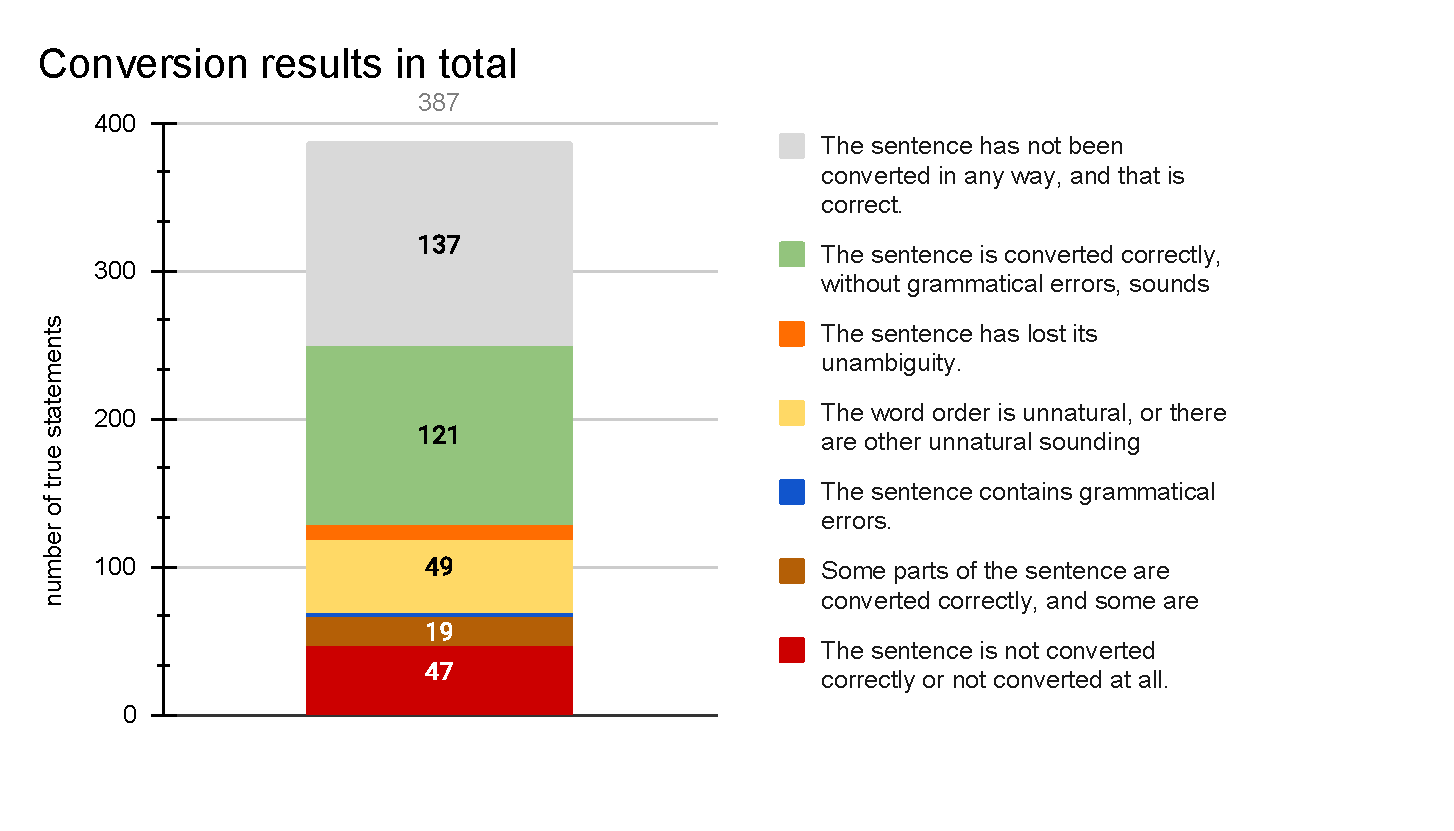
\includegraphics[width=\textwidth]{data/Eval-Total.pdf}
\caption{Results statistics in total}
\label{fig:eval-total}
\end{figure}

Now let us take a look at the results for each narrative mode.

\subsection{First-person to Third-person results}

Figure \ref{fig:eval-first-to-third} shows very good results for the first-person narrative to third-person narrative conversion. Less than 5\% of the sentences were converted partially or completely incorrectly. Moreover, about 82\% of the remaining sentences were converted (or not converted) without any quality loss. The most common problem was unnatural word order.

\begin{figure}[!ht]
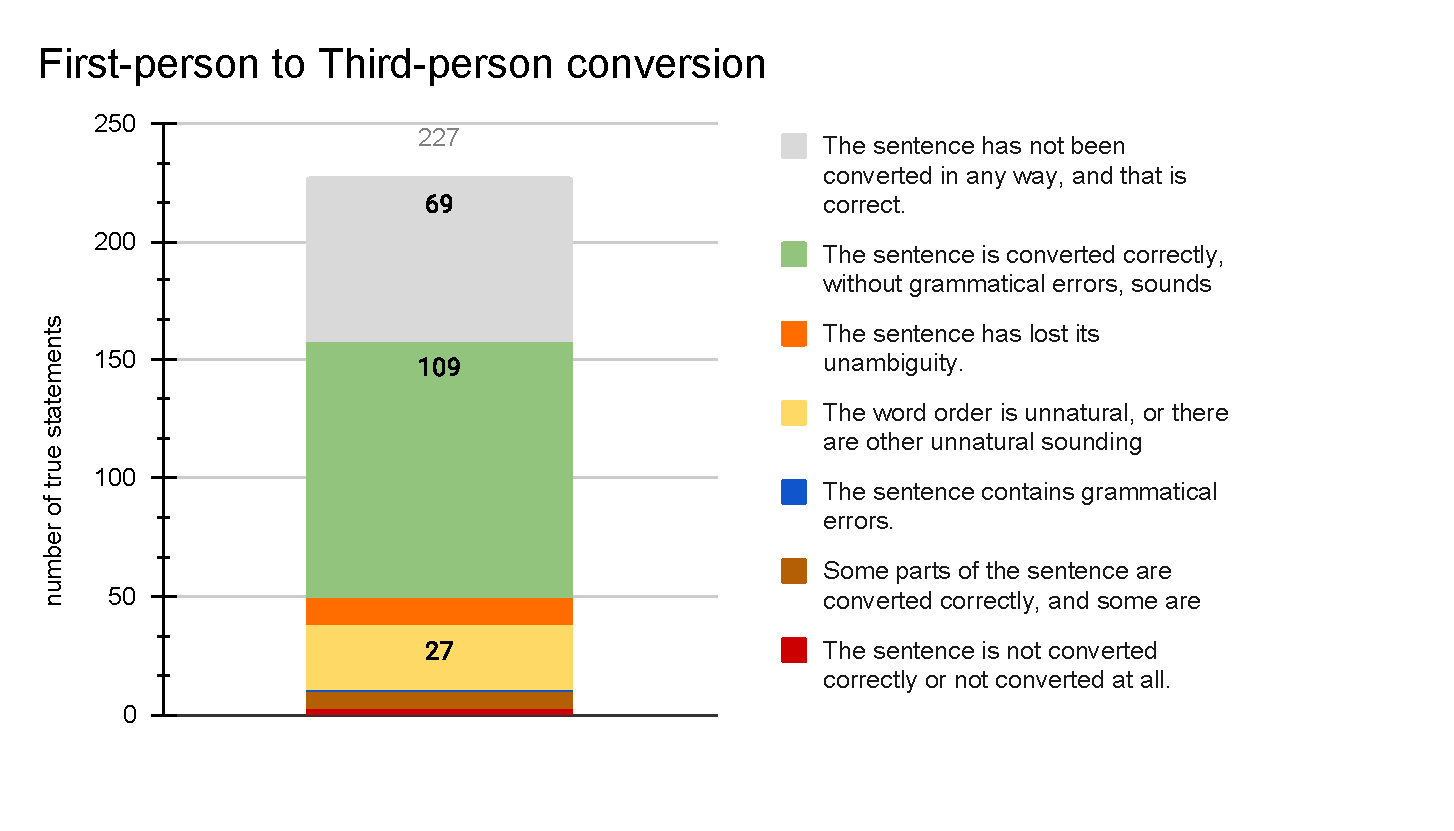
\includegraphics[width=\textwidth]{data/Eval-First-To-Third.pdf}
\caption{Results statistics for first-person to third-person conversion}
\label{fig:eval-first-to-third}
\end{figure}



\subsection{Third-person to First-person results}
On the other hand, figure \ref{fig:eval-third-to-first} illustrates quite a different picture. The third-to-first conversion direction delivers poor performance results. Notice that the number of completely incorrect sentences is very high (more than 25\%) even when considering the fact that 68 sentences were not affected by the conversion at all.
The reasons for these poor results are further described in Section \ref{sec:errors}.

\begin{figure}[!ht]
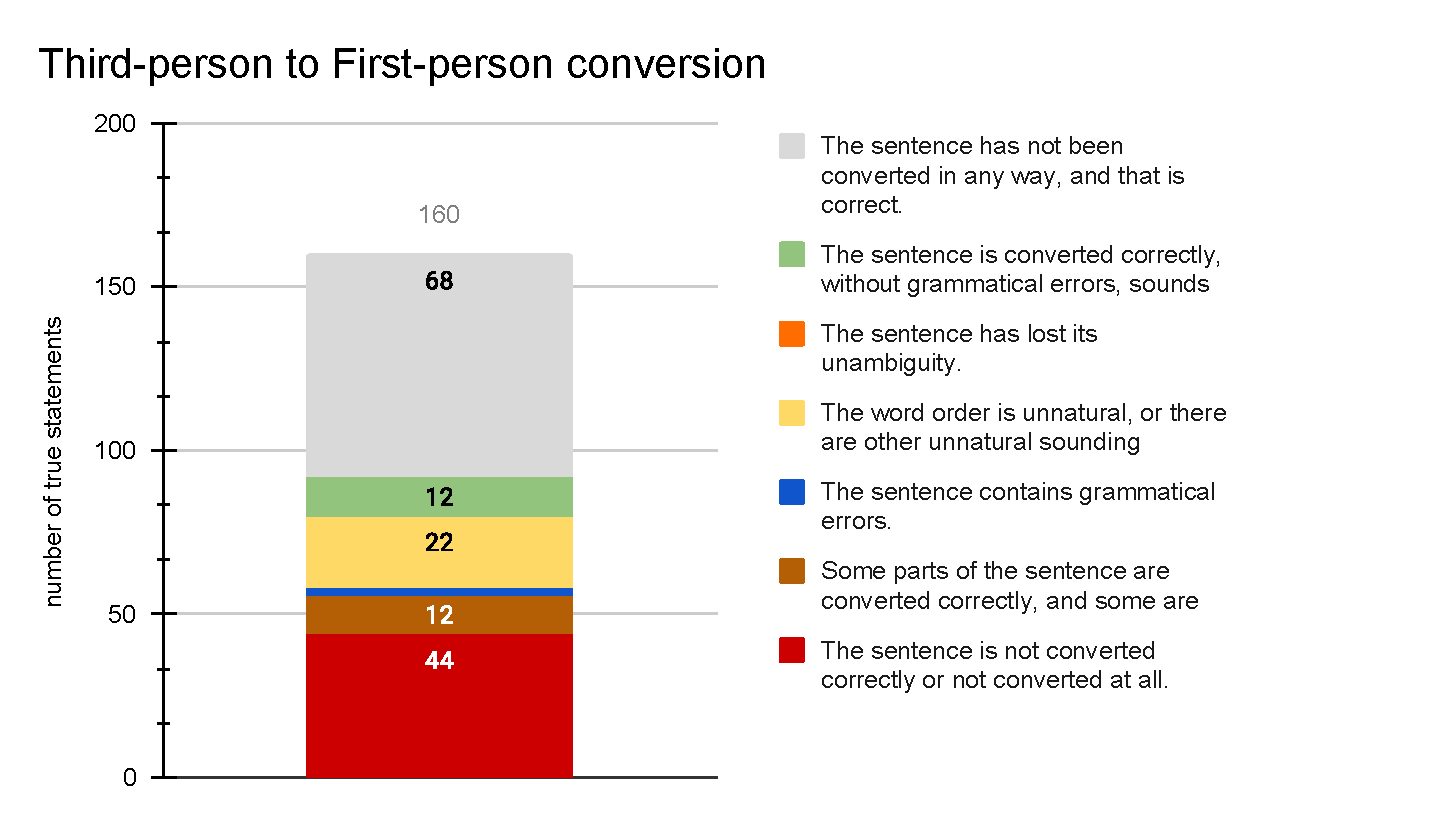
\includegraphics[width=\textwidth]{data/Eval-Third-To-First.pdf}
\caption{Results statistics for third-person to first-person conversion}
\label{fig:eval-third-to-first}
\end{figure}

\section{Errors and How to Fix Them} \label{sec:errors}

In this section, I provide an error analysis. I examine the causes of the errors and discuss their solvability. The errors are divided into two groups: 1) incorrect conversion and 2) text quality lost.

\subsection{Conversion Errors}

As mentioned in the previous section, most conversion errors come from the third-to-first conversion. Since this direction is much more complicated than the other way, the poorer results are not surprising. In contrast to first-to-third, when converting a text from the third-person narrative, we need to recognize the protagonist who should become the narrator and change all the words whose form depends on this protagonist. This task should be handled by anaphora resolution. Nevertheless, the performance of Aara is poor. Thus, it affects RephrasErIch. The considerable difference between first-to-third and third-to-first results confirms this issue since anaphora resolution is not used in the first-to-third conversion.

A solution to this error is beyond the limits of the tool. Aara would have to be improved or replaced by better performing tool.

\subsection{Text Quality Errors}

\subsubsection{Word order}

Unnatural word order is the most common quality error. It was usually caused by adding or removing words during the conversion. It mostly includes:

\begin{itemize}
	\item \textbf{Adding or removing a subject.} Example: \emph{Adam věří jim to.} The original sentence here was \emph{Věřím jim to.} and the tool added the protagonist's name at the beginning of the sentence. However, the other words should be reordered to sound natural: \emph{Adam jim to věří.}
	\item \textbf{Adding or removing an auxiliary verb.} Example: \emph{Konečně se jsem mohla rozesmát.} The auxiliary verb \emph{jsem} was added to the original sentence \emph{Konečně se mohla rozesmát.}. In Czech, it is natural for reflexive pronoun \emph{se} to come after the auxiliar: \emph{Konečně jsem se mohla rozesmát.}
\end{itemize}

Word order in Czech sentences is relatively free, but some strict rules exist. Implementing these rules into the system would solve many unnaturally sounding sentences.

Nevertheless, the order might be chosen according to other factors, such as emotional state, communication aim of the speaker, etc. These factors can not be easily expressed in rules.


\subsubsection{Prepositions}

Some prepositions in the Czech language have a shorter and longer version. The longer versions aim to make the pronunciation easier. There is no official rule saying when to use which, but the longer versions are usually used to make the pronunciation easier.

Right now, the tool does not change the preposition during the conversion. The evaluation revealed this as a problem that creates unnaturally sounding phrases.

For instance, let us have a sentence \emph{Táta šel k ní}. Converting the sentence to the first-person narrative, we get \emph{Táta šel k mně}. However, that is unnatural, and it is harder to pronounce -- we would rather write \emph{Táta šel ke mně}. This also applies in vice versa.

I suppose this issue could be solvable by adding a few rules. As has been said, no official rule for this exists, but there are some general common-sense rules to apply.

\subsubsection{Proper nouns vs. pronouns}

- použití vlastního jména vs. použití zájmena, pozice ve větě

\subsubsection{Unambiguity}

- jednoznačnost -- first-to-third --> zmenou osoby neni jasné, na koho treba zajmeno odkazuje, kdo to dela atd.

TODO TODO TODO



